\documentclass[journal,12pt,twocolumn]{IEEEtran}
\usepackage[utf8]{inputenc}
\usepackage{amsmath}
\usepackage{amssymb}
\usepackage{enumerate}
\usepackage{mathtools}
%\usepackage{graphicx}
\usepackage{multicol}
\usepackage{caption}
\usepackage{iithtlc}
%\usepackage[font=scriptsize]{caption}
%\graphicspath{{/home/shweta/Documents/relatex23/RLC}}


\begin{document}
\title{
	\logo{
	Gate Problems on Circuit Analysis
	}
%		Signals \& Circuits
}
% make the title area
\maketitle

%\tableofcontents

\bigskip

\begin{abstract}
%\boldmath
This problem set has questions related to RLC circuits taken from GATE papers over the last twenty years.  Teachers can use the problem set for course tutorials. 
 
\end{abstract}

\begin{enumerate}
\setlength\itemsep{2em}


\item  In a series RLC high Q circuit,the current peaks at a frequency
\begin{enumerate}
\setlength\itemsep{1em}
\item Equal to the resonant frequency.
\item Greater than the resonant frequnecy.
\item Less than the resonant frequency.
\item None of the above.
\end{enumerate}


\item The network shown in figure.\ref{fig1} is initially under steady state condition with the switch in position1.The switch is moved from position1 to position2 at $t\neq0$.Calculate the current i(t) through R$_{1}$ after switching. 

\begin{figure}[!h]
\begin{center}
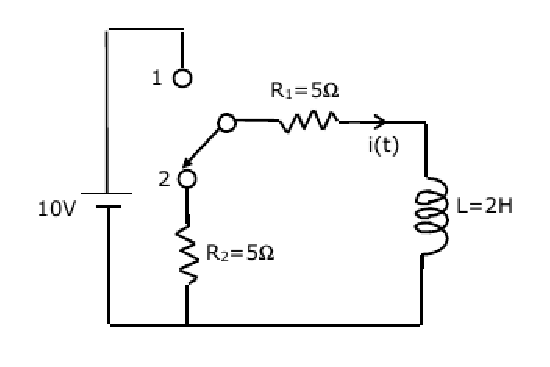
\includegraphics[scale=0.5]{./figs/fig1.eps}
\caption{}
\label{fig1}
\end{center}  
\end{figure}

\item For the series R-L circuit of figure(a)\ref{fig2}, the partial fissure diagram at a certain
frequency is shown in figure(b).The operating frequency of the circuit is:
\begin{enumerate}
\setlength\itemsep{1em}
\item Equal to the resonance frequency.
\item Less than the resonance frequency.
\item Greater than resonance frequency.
\item Not zero.
\begin{figure}[!h]
\begin{center}
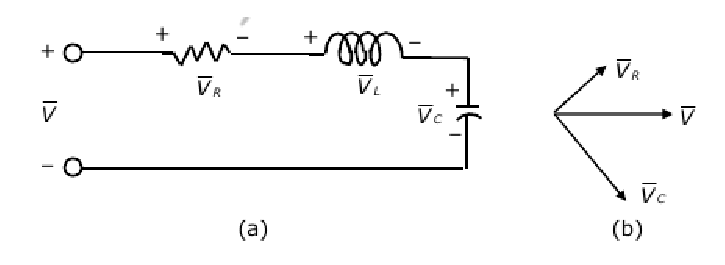
\includegraphics[scale=0.5]{./figs/fig2.eps}
\caption{}
\label{fig2}
\end{center}
\end{figure}
\end{enumerate}


\item For the compensated attenuator of figure\ref{fig3}, the impulse response under the
condition R$_{1}C_{1}$ = R$_{2}C_{2}$  is:
\begin{figure}[!h]
\begin{center}

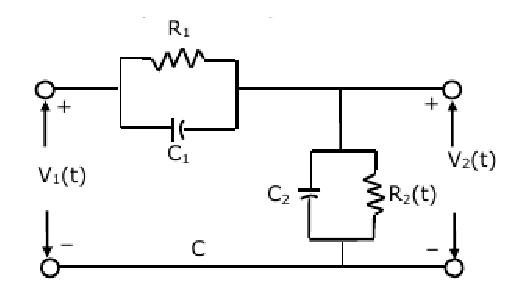
\includegraphics[scale=0.5]{./figs/fig3.eps}
\caption{}
\label{fig3}
\end{center}
\end{figure}
\begin{enumerate}
\setlength\itemsep{2em}
\item $\frac{R_2}{{R_1}+R_2}\big[{1-{e^{\frac{1}{R_1C_1}}}}\big]$u(t)
\item $\frac{R_2}{{R_1}+R_2}\delta$(t)
\item $\frac{R_2}{{R_1}+R_2}$ u(t)
\item $\frac{R_2}{{R_1}+R_2}{1-{e^{\frac{1}{R_1C_1}}}}$u(t)
\end{enumerate}

\item Of the four networks N$_{1}$,N$_{2}$,N$_{3}$ and N$_{4}$ of figure\ref{fig4}, the networks having identical
driving point functions are
\begin{enumerate}
\begin{multicols}{2}
\setlength\itemsep{2em}
\item $N_1 and N_1$
\item $N_2 and N_4$
\item $N_1 and N_3$
\item $N_1 and N_4$
\end{multicols}
\begin{figure}[!h]

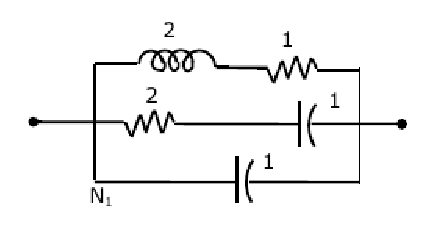
\includegraphics[scale=0.5]{./figs/fig4a.eps}
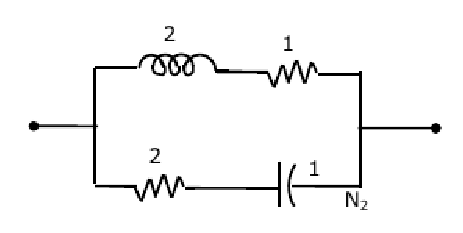
\includegraphics[scale=0.5]{./figs/fig4b.eps}
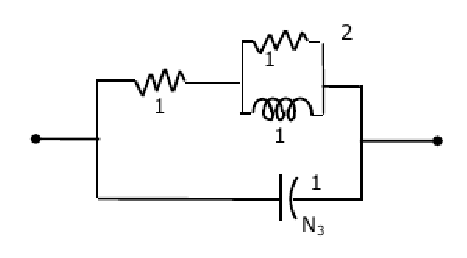
\includegraphics[scale=0.5]{./figs/fig4c.eps}
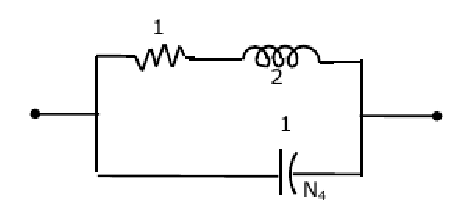
\includegraphics[scale=0.5]{./figs/fig4d.eps}
\caption{}
\label{fig4}
\end{figure}
\end{enumerate}


\item In the series circuit shown in figure.\ref{fig5} for series resonance,the value of the
coupling coefficient K will be
\begin{enumerate}
\begin{multicols}{4}
\setlength\itemsep{2em}
\item 0.25
\item 0.5
\item 0.999
\item 1.0
\end{multicols}
\begin{figure}[!h]
\begin{center}

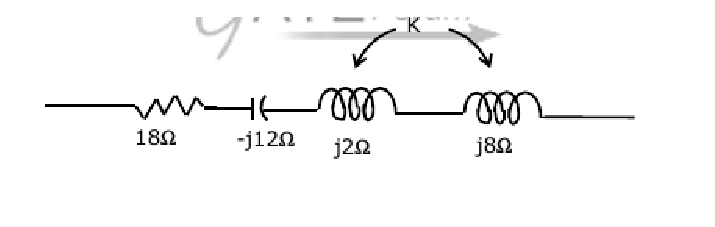
\includegraphics[scale=0.5]{./figs/fig5.eps}
\caption{}
\label{fig5}
\end{center}
\end{figure}
\end{enumerate}


\item In the circuit of figure.\ref{fig6}, when switch S$_{1}$ is closed,the ideal ammeter M$_{1}$ reads 5A.What will be ideal voltmeter M$_{2}$ read when S$_{1}$ is kept open?(The value of E is not specified).
\begin{figure}[!h]
\begin{center}
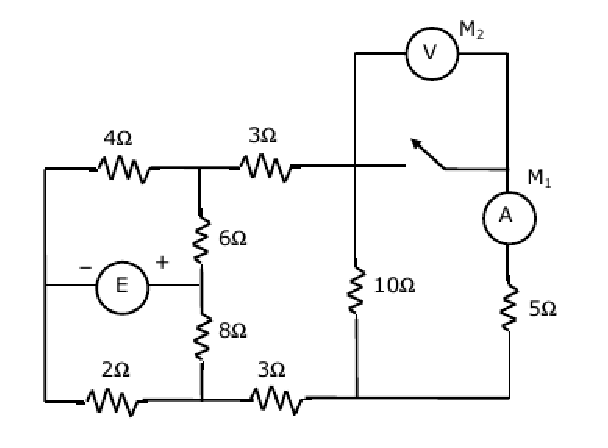
\includegraphics[scale=0.7]{./figs/fig6.eps}
\caption{}
\label{fig6}
\end{center}
\end{figure}

\item In figure.\ref{fig7} A$_{1}$,A$_{2}$andA$_{3}$ are ideal ammeters?If A$_{1}$ reads 5A,A$_{2}$ reads 12A, then A$_{3}$ should read.
\begin{enumerate}
\begin{multicols}{4}
\setlength\itemsep{2em}
\item 7A
\item 12A
\item 13A
\item 17A
\end{multicols}
\begin{figure}[!h]
\begin{center}
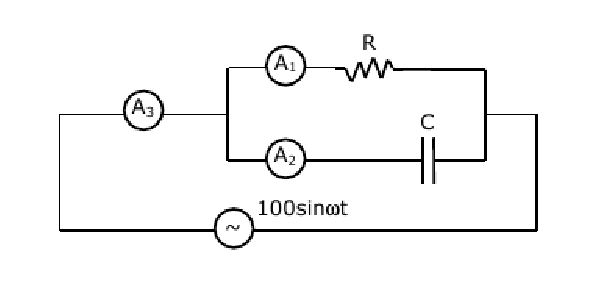
\includegraphics[scale=0.7]{./figs/fig7.eps}
\caption{}
\label{fig7}
\end{center}
\end{figure}
\end{enumerate}

\item Find the Y-parameters(short circuit admittance parameters)for the network shown in figure.\ref{fig8}
\begin{figure}[!h]
\begin{center}
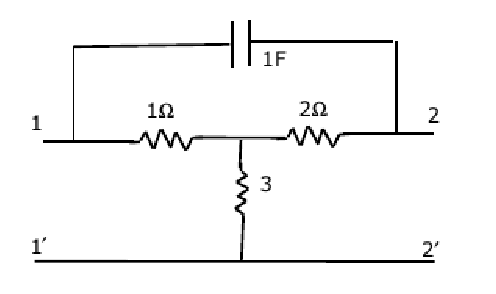
\includegraphics[scale=0.5]{./figs/fig8.eps}
\caption{}
\label{fig8}
\end{center}
\end{figure}


\item The voltages V$_{c1}$,V$_{c2}$ and V$_{c3}$ across the capacitors in the circuit in the given figure\ref{fig9},under steady state are respectively
\begin{enumerate}
\setlength\itemsep{2em}
\begin{multicols}{2}
\item 80V,32V,48V
\item 80V,48V,32V
\item 20V,8V,12V
\item 20V,12V,8V
\end{multicols}
\begin{figure}[!h]
\begin{center}
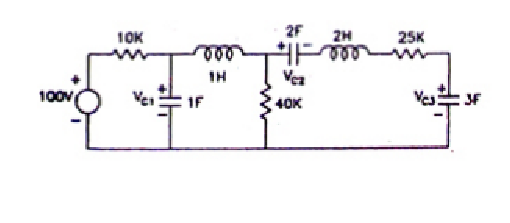
\includegraphics[scale=0.7]{./figs/fig9.eps}
\caption{}
\label{fig9}
\end{center}
\end{figure}
\end{enumerate}

\item In the circuit shown in figure\ref{fig10} is (a)-(c),assuming initial voltage and capacitors and currents through the inductors to be zero at the time of switching(t=0),then at anytime $t>0$
\begin{enumerate}
\setlength\itemsep{2em}
\item Current increases monotonically with time
\item Current decreases monotonically with time
\item Current remains constant at V/R
\item Current first increases then decreases
\item No current can ever flow
\begin{figure}[!h]
\begin{center}
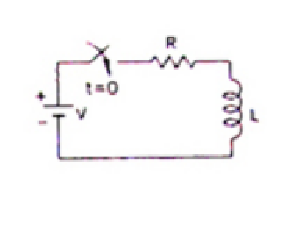
\includegraphics[scale={0.7}]{./figs/fig10a.eps}
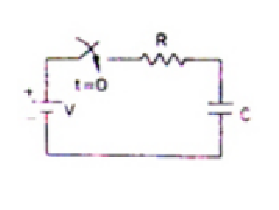
\includegraphics[scale={0.7}]{./figs/fig10b.eps}
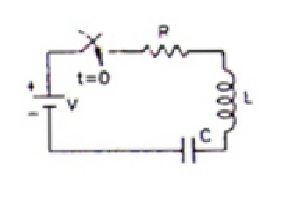
\includegraphics[scale={0.7}]{./figs/fig10c.eps}
\caption{}
\label{fig10}
\end{center}
\end{figure}
\end{enumerate}

                   
              
\item The current $i_{4}$ in the circuit of the figure\ref{fig11} is equal to
\begin{enumerate}
\setlength\itemsep{2em}
\begin{multicols}{4}
\item 12A
\item -12A
\item 4A
\item None of these
\end{multicols}
\begin{figure}[!h]
\begin{center}
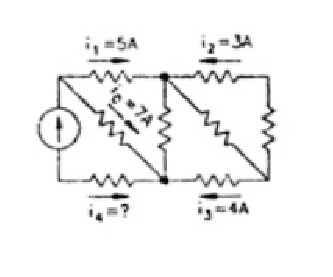
\includegraphics[scale=0.7]{./figs/fig11.eps}
\caption{}
\label{fig11}
\end{center}
\end{figure}
\end{enumerate}
       
       
\item The voltage V in the figure\ref{fig12} is equal to
\begin{enumerate}
\setlength\itemsep{2em}
\begin{multicols}{4}
\item 3V
\item -3V
\item 5V
\item None of these
\end{multicols}
\begin{figure}[!h]
\begin{center}
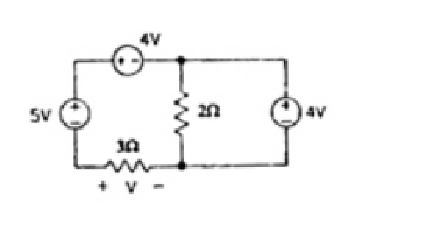
\includegraphics[scale=0.7]{./figs/fig12.eps}
\caption{}
\label{fig12}
\end{center}
\end{figure}
\end{enumerate}


\item The voltage V in the figure\ref{fig13} is always equal to
\begin{enumerate}
\setlength\itemsep{2em}
\begin{multicols}{4}
\item 9V
\item 5V
\item 1V
\item None of these
\end{multicols}
\begin{figure}[!h]
\begin{center}
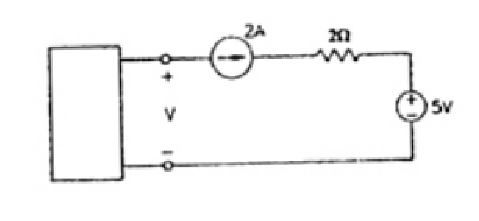
\includegraphics[scale=0.5]{./figs/fig13.eps}
\caption{}
\label{fig13}
\end{center}
\end{figure}
\end{enumerate}


\item The voltage V in the figure\ref{fig14} is 

\begin{enumerate}
\setlength\itemsep{2em}
\begin{multicols}{2}
\item 10V
\item 15V
\item 5V
\item None of these
\end{multicols}
\begin{figure}[!h]
\begin{center}
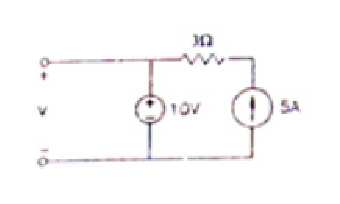
\includegraphics[scale=0.7]{./figs/fig14.eps}
\caption{}
\label{fig14}
\end{center}
\end{figure}

\end{enumerate}


\item In the circuit of the figure\ref{fig15} is the energy absorbed by the $4\Omega$ resistor in the time interval (0,$\infty$) is
\begin{figure}[!h]
\begin{center}
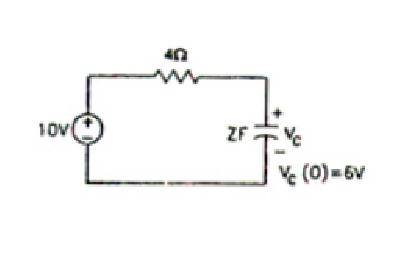
\includegraphics[scale=0.7]{./figs/fig15.eps}
\caption{}
\label{fig15}
\end{center}
\end{figure}

\begin{enumerate}
\setlength\itemsep{2em}
\begin{multicols}{2}
\item 36 Joules
\item 16 Joules
\item 256 Joules
\item None of these
\end{multicols}

\end{enumerate}


\item In the circuit of the figure\ref{fig16} is the equivalent impedance seen across terminals a,b is
\begin{enumerate}
\setlength\itemsep{2em}
\begin{multicols}{2}
\item $\big(\frac{16}{3}\big)\Omega$
\item $\big(\frac{8}{3}\big)\Omega$
\item $\big(\frac{8}{3}+12j\big)\Omega$
\item None of above
\end{multicols}
\begin{figure}[!h]
\begin{center}
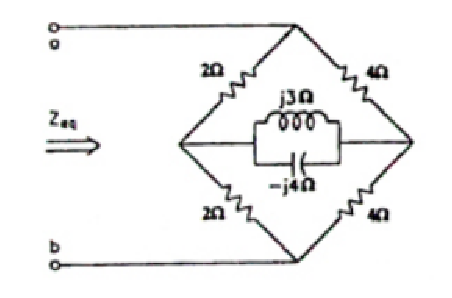
\includegraphics[scale=0.9]{./figs/fig16.eps}
\caption{}
\label{fig16}
\end{center}
\end{figure}
\end{enumerate}


\item A communication channel has first order low pass transfer function.The channel is used to transmit pulses at a symbol rate greater than the half-power frequency of the low pass function.Which of the network shown in the figure\ref{fig17} is can be used to equalise the received pulses?
\begin{figure}[!h]
\begin{center}
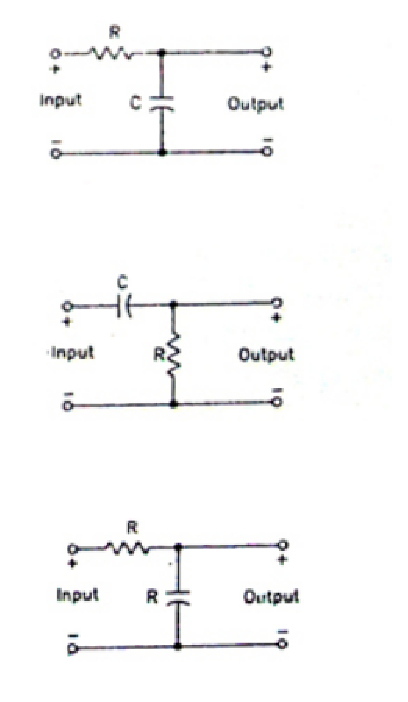
\includegraphics[scale=0.8]{./figs/fig17.eps}
\caption{}
\label{fig17}
\end{center}  
\end{figure}


\item In the circuit of the figure\ref{fig18} is R=100$\Omega$,L=20 nH and C=32pF.The circuit is maintained at a temperature of 300k.Derive and plot the power spectral density of the voltage $V_{0}$.Mark all the relevant points on the plot with numerical values.(The Boltzmann constant k=1.28$\times$10-23J/k)
\begin{figure}[!h]
\begin{center}
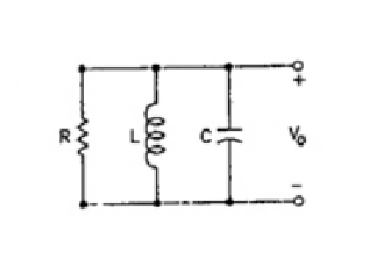
\includegraphics[scale=0.5]{./figs/fig18.eps}
\caption{}
\label{fig18}
\end{center}  
\end{figure}


\item In the circuit of figure\ref{fig19} when R=0$\Omega$,the current $i_{k}$ equals 10A
\begin{enumerate}
\setlength\itemsep{2em}
\item Find the value of R for which it absorbs maximum power
\item Find the value of $\varepsilon$
\item Find $V_{2}$ when R=$\infty$(open circuit)
\begin{figure}[!h]
\begin{center}
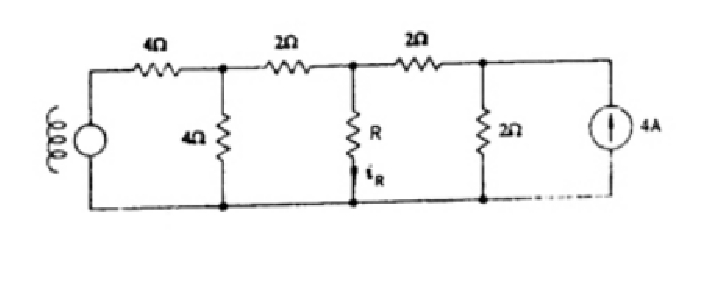
\includegraphics[scale=0.5]{./figs/fig19.eps}
\caption{}
\label{fig19}
\end{center}
\end{figure}
\end{enumerate}


\item In the circuit of the figure.\ref{fig20} is all currents and voltages are sinusoids of frequency $\omega$ rad/sec.
\begin{enumerate}
\setlength\itemsep{2em}
\item Find the impedance to the right of(A,B) at $\omega$=0 rad/sec and $\omega$=$\infty$ rad/sec.
\item if $\omega=\omega_{0}$ rad/sec and $i_{1}$(t)=I sin($\omega_{0}$t) A,where I is positive $\omega_{0}\neq$0 ,$\omega_{0}\neq\infty$ then find I,$\omega_{0}$ and $i_{2}$(t)
\begin{figure}[!h]
\begin{center}
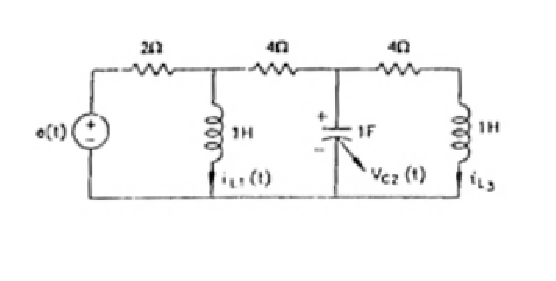
\includegraphics[scale=0.5]{./figs/fig20.eps}
\caption{}
\label{fig20}
\end{center}
\end{figure}
\end{enumerate}


\item The nodal method of circuit analysis is based on
\begin{enumerate}
\setlength\itemsep{2em}
\item KVL and Ohm's law
\item kCL and Ohm's law
\item KCL and KVL
\item KCL,KVL and Ohm's law
\end{enumerate}


\item Superposition theorem is NOT applicable to networks containing
\begin{enumerate}
\setlength\itemsep{2em}
\item Nonlinear elements
\item Dependent Voltage Sources
\item Dependent current sources
\item transformers
\end{enumerate}

\item The parallel RLC circuit shown in figure.\ref{fig21} is in resonance.In this circuit
\begin{enumerate}
\setlength\itemsep{2em}
\begin{multicols}{2}
\item $\vert$I$_{R}\vert<$1mA
\item $\vert$I$_{R}+$I$_{L}\vert>$1mA
\item $\vert$I$_{R}+$I$_{C}\vert<$1mA
\item $\vert$I$_{R}+$I$_{C}\vert>$1mA
\end{multicols}
\begin{figure}[!h]
\begin{center}
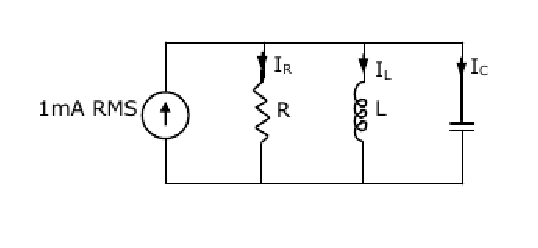
\includegraphics[scale=0.5]{./figs/fig21.eps}
\caption{}
\label{fig21}
\end{center}
\end{figure}
\end{enumerate}

\item The Voltage across the terminals a and b in figure.\ref{fig22} is
\begin{enumerate}
\setlength\itemsep{2em}
\begin{multicols}{4}
\item 0.5V
\item 3.0V
\item 3.5V
\item 4.0V
\end{multicols}
\begin{figure}[!h]
\begin{center}
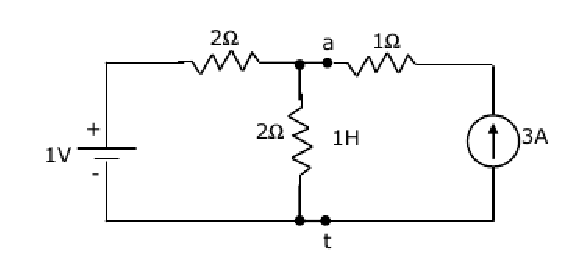
\includegraphics[scale=0.5]{./figs/fig22.eps}
\caption{}
\label{fig22}
\end{center}
\end{figure}
\end{enumerate}

\item Determine the frequency of resonance and the resonant impedance of the parallel circuit shown in Figure.\ref{fig23}.What happens when L = $CR^{2}$ ?
\begin{figure}[!h]
\begin{center}
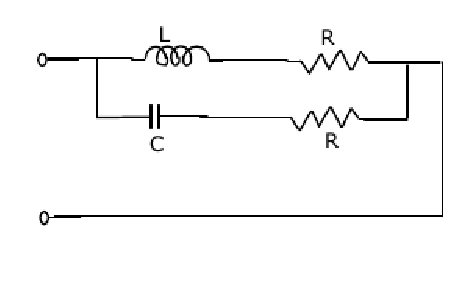
\includegraphics[scale=0.5]{./figs/fig23.eps}
\caption{}
\label{fig23}
\end{center}
\end{figure}


\item The Thevenin equivalent voltage V$_{TH}$appearing between the terminals A and B of
the network shown in Fig.\ref{fig24} is given by
\begin{enumerate}
\setlength\itemsep{2em}
\begin{multicols}{2}
\item j16(3-j4)
\item j16(3+j4)
\item 16(3+j4)
\item 16(3-j4)
\end{multicols}
\begin{figure}[!h]
\begin{center}
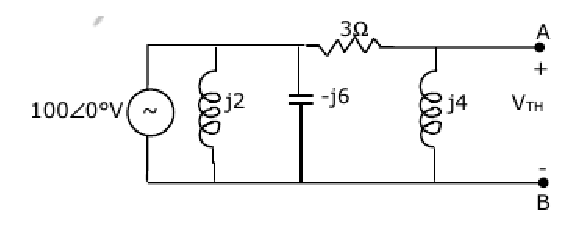
\includegraphics[scale=0.5]{./figs/fig24.eps}
\caption{}
\label{fig24}
\end{center}
\end{figure}
\end{enumerate}

\item The value of R (in ohms) required for maximum power transfer in the network
shown in Fig.\ref{fig25} is
\begin{enumerate}
\setlength\itemsep{2em}
\begin{multicols}{4}
\item 2
\item 4
\item 8
\item 10
\end{multicols}
\begin{figure}[!h]
\begin{center}
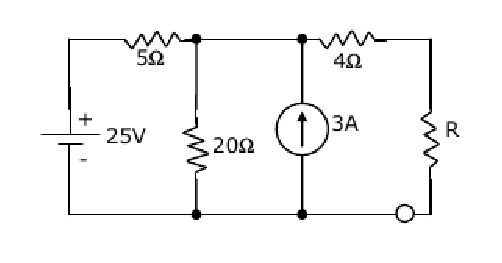
\includegraphics[scale=0.5]{./figs/fig25.eps}
\caption{}
\label{fig25}
\end{center}
\end{figure}
\end{enumerate}


\item A Delta-connected network with its Wye-equivalent is shown in Fig\ref{fig26},fig\ref{fig27}.The resistance $R_{1}$,$R_{2}$ and $R_{3}$  (in ohms) are respectively
\begin{figure}[!h]
\begin{center}
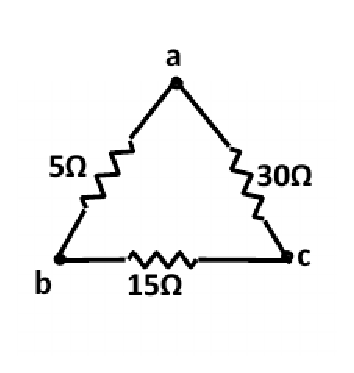
\includegraphics[scale=0.5]{./figs/fig26.eps}
\caption{}
\label{fig26}
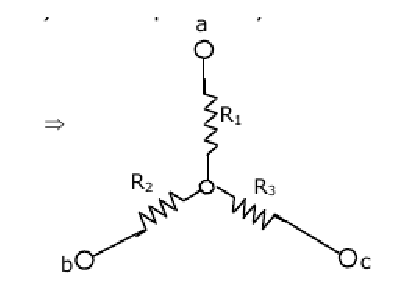
\includegraphics[scale=0.5]{./figs/fig27.eps}
\caption{}
\label{fig27}
\end{center}
\end{figure}


\item In the circuit of Fig.\ref{fig28},the switch 'S' has remained open for a long time. The switch closes instantaneously at t=0
\begin{enumerate}
\setlength\itemsep{2em}
\item Find $V_{0}$ for t$\leq$0 and as t$\rightarrow\infty$
\item Write an expression for $V_{0}$ as function of time for 0$\leq$t$\leq\infty$
\item Evaluate $V_{0}$ at t=25 $\mu$sec
\begin{figure}[!h]
\begin{center}
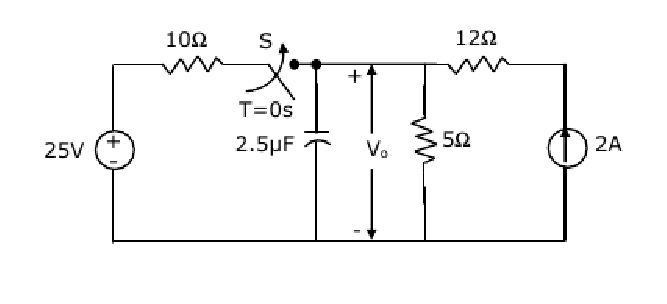
\includegraphics[scale=0.5]{./figs/fig28.eps}
\caption{}
\label{fig28}
\end{center}
\end{figure}
\end{enumerate}

\item For the network shown in Fig.\ref{fig29} evaluate the  current I flowing through the 2$\Omega$ resistor using superposition theorem.
\begin{figure}[!h]
\begin{center}
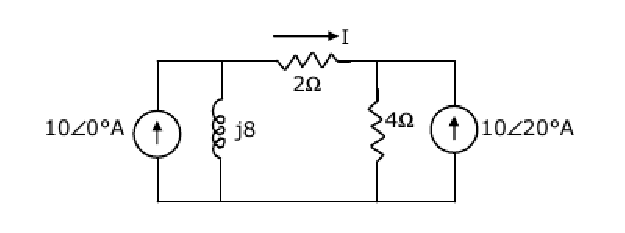
\includegraphics[scale=0.5]{./figs/fig29.eps}
\caption{}
\label{fig29}
\end{center}
\end{figure}


\item In the circuit of Fig.\ref{fig30} the voltage v(t)is
\begin{figure}[!h]
\begin{center}
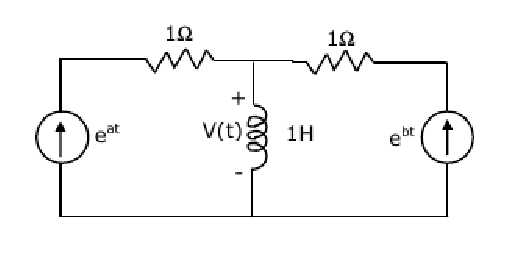
\includegraphics[scale=0.5]{./figs/fig30.eps}
\caption{}
\label{fig30}
\end{center}
\end{figure}

\begin{enumerate}
\setlength\itemsep{2em}
\begin{multicols}{2}
\item $e^{at}$-$e^{bt}$
\item $e^{at}$+$e^{bt}$
\item $ae^{at}$-$be^{bt}$
\item $ae^{at}$+$be^{bt}$
\end{multicols}

\end{enumerate}

\item The circuit of figure.\ref{fig31} represents a
\begin{enumerate}
\setlength\itemsep{2em}
\begin{multicols}{2}
\item low pass filter
\item high pass filter
\item band pass filter
\item band reject filter
\end{multicols}
\begin{figure}[!h]
\begin{center}
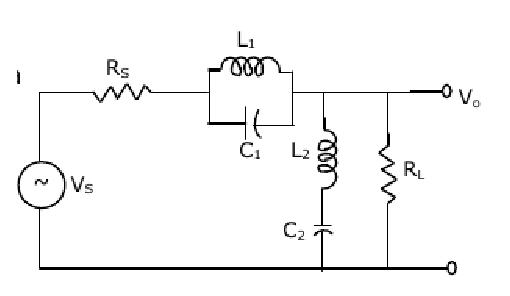
\includegraphics[scale=0.5]{./figs/fig31.eps}
\caption{}
\label{fig31}
\end{center}
\end{figure}
\end{enumerate}

\item Use the data of figure.\ref{fig32} .The current I in the circuit of figure(b) is
\begin{enumerate}
\setlength\itemsep{2em}
\begin{multicols}{4}
\item -2A
\item 2A
\item -4A
\item +4A
\end{multicols}
\begin{figure}[!h]
\begin{center}
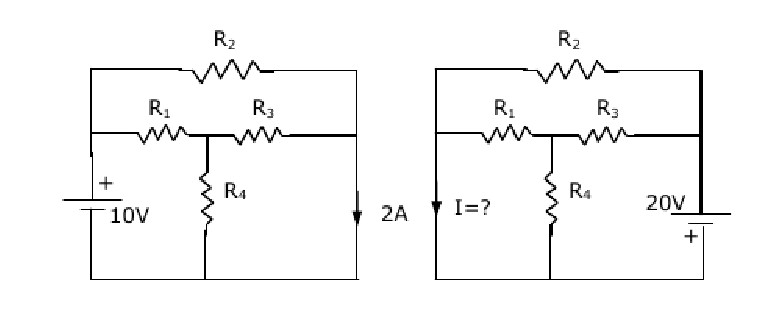
\includegraphics[scale=0.5]{./figs/fig32.eps}
\caption{}
\label{fig32}
\end{center}
\end{figure}
\end{enumerate}

\item For the circuit in figure.\ref{fig33}
\begin{enumerate}
\setlength\itemsep{2em}
\item Find the Thevenin equivalent of the sub circuit faced by the capacitor across
the terminals a,b.
\item Find $v_{c}$(t),t$>$0,given $V_{c}$(0)=0
\item Find i(t),t$>$0
\begin{figure}[!h]
\begin{center}
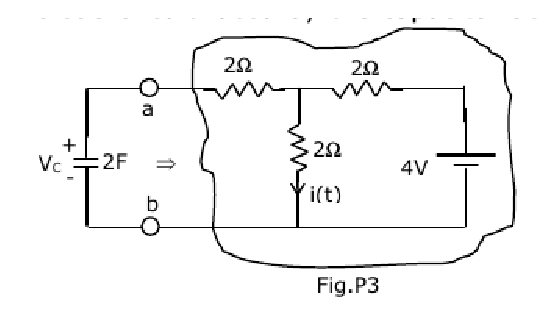
\includegraphics[scale=0.5]{./figs/fig33.eps}
\caption{}
\label{fig33}
\end{center}
\end{figure}
\end{enumerate}

\item For the circuit in figure\ref{fig34},which is in steady state.
\begin{enumerate}
\setlength\itemsep{2em}
\item Find the frequency $\omega_{0}$ at which the magnitude of the impedance across
terminals a,b reaches a maximum.
\item Find the impedance across a,b at the frequency $\omega_{0}$.
\item if $v_{s}$(t)=V sin($\omega_{0}$t),find $i_{L}$(t),$i_{R}$(t).
\begin{figure}[!h]
\begin{center}
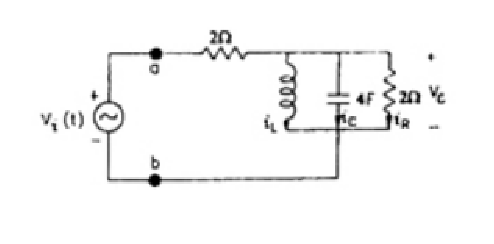
\includegraphics[scale=0.9]{./figs/fig34.eps}
\caption{}
\label{fig34}
\end{center}
\end{figure}
\end{enumerate}

\item For the circuit in figure\ref{fig35},write the state equations using $v_{c}$ and $i_{L}$ as state variables
\begin{figure}[!h]
\begin{center}
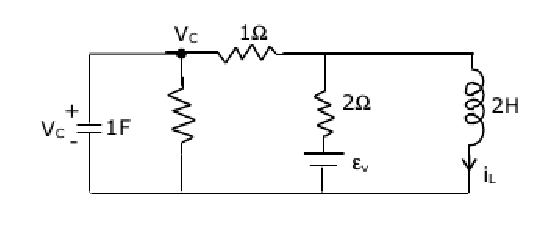
\includegraphics[scale=0.5]{./figs/fig35.eps}
\caption{}
\label{fig35}
\end{center}
\end{figure}


\item The voltage $e_{0}$ in figure\ref{fig36} is
\begin{enumerate}
\setlength\itemsep{2em}
\begin{multicols}{4}
\item 2V
\item $\frac{4}{3}$ V
\item 4V
\item 8V
\end{multicols}
\begin{figure}[!h]
\begin{center}
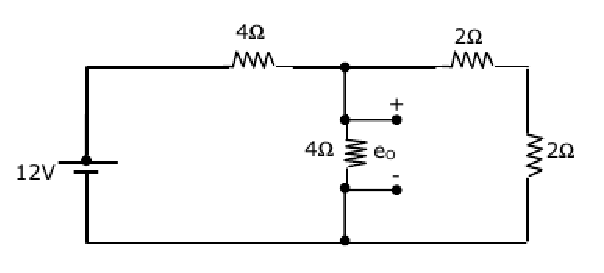
\includegraphics[scale=0.5]{./figs/fig36.eps}
\caption{}
\label{fig36}
\end{center}
\end{figure}
\end{enumerate}

\item The voltage $e_{0}$ in figure\ref{fig37} is
\begin{enumerate}
\setlength\itemsep{2em}
\begin{multicols}{4}
\item 48V
\item 24V 
\item 36V
\item 28V
\end{multicols}
\begin{figure}[!h]
\begin{center}
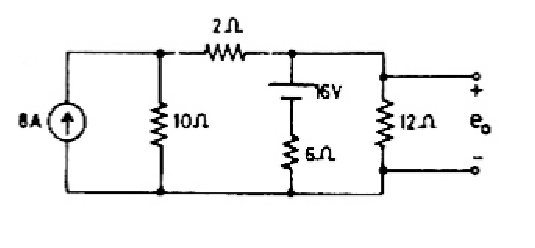
\includegraphics[scale=0.5]{./figs/fig37.eps}
\caption{}
\label{fig37}
\end{center}
\end{figure}
\end{enumerate}

\item In figure\ref{fig38},the value of the load resistor R which maximizes the power delivered to it is
\begin{enumerate}
\setlength\itemsep{2em}
\begin{multicols}{2}
\item 14.14$\Omega$
\item 10$\Omega$
\item 200$\Omega$
\item 28.28$\Omega$
\end{multicols}
\begin{figure}[!h]
\begin{center}
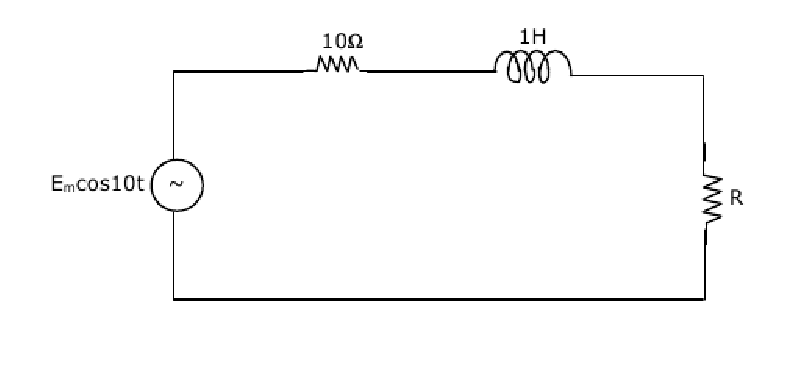
\includegraphics[scale=0.5]{./figs/fig38.eps}
\caption{}
\label{fig38}
\end{center}
\end{figure}
\end{enumerate}

\item When the angular frequency $\omega$ in Figure\ref{fig39} is varied from 0 to $\infty$, the locus of the current phasor$ I_{2}$ is given by
\begin{figure}[!h]
\begin{center}
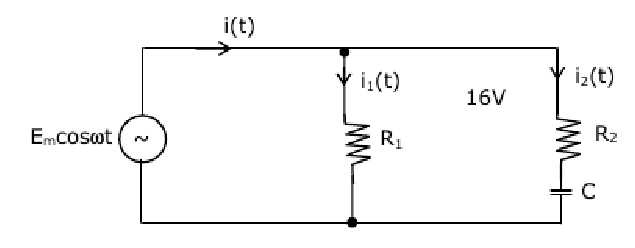
\includegraphics[scale=0.5]{./figs/fig39a.eps}
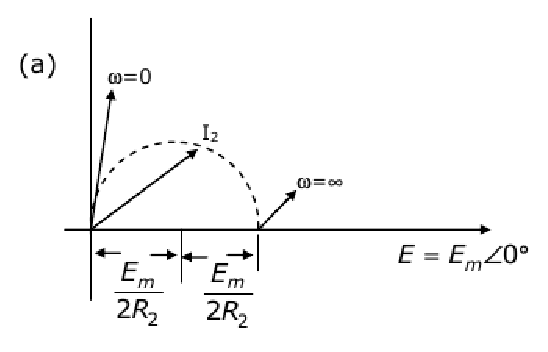
\includegraphics[scale=0.5]{./figs/fig39b.eps}
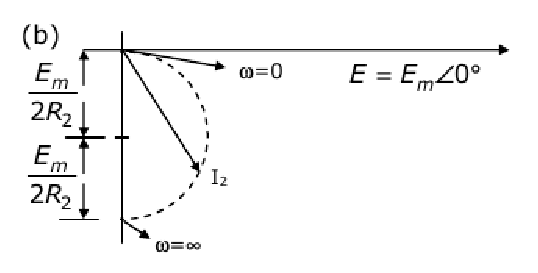
\includegraphics[scale=0.5]{./figs/fig39c.eps}
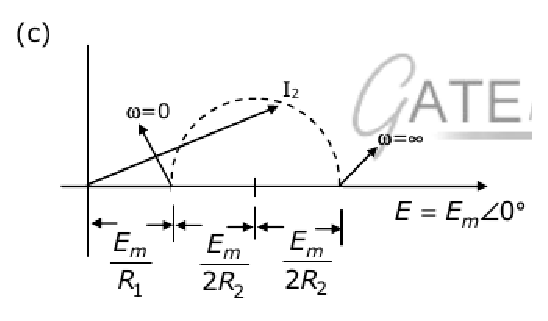
\includegraphics[scale=0.5]{./figs/fig39d.eps}
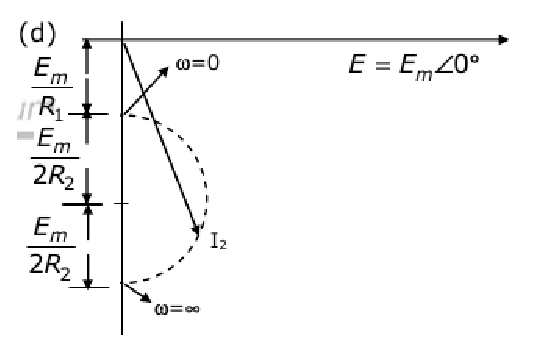
\includegraphics[scale=0.5]{./figs/fig39e.eps}
\caption{}
\label{fig39}
\end{center}
\end{figure}

\item For the circuit shown in figure\ref{fig40},determine the phasors $E_{2}$,$E_{0}$,I and $I_{1}$
\begin{figure}[!h]
\begin{center}
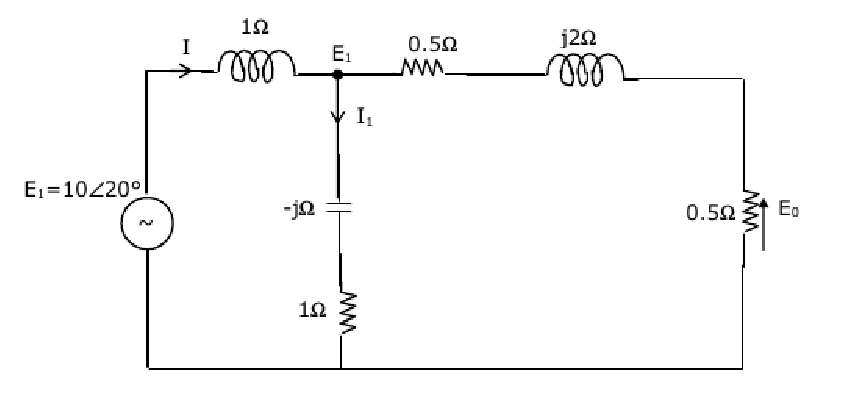
\includegraphics[scale=0.3]{./figs/fig40.eps}
\caption{}
\label{fig40}
\end{center}
\end{figure}

\item The circuit shown in figure\ref{fig41} is operating in steady-state with switch $S_{1}$ closed. 
\begin{enumerate}
\setlength\itemsep{2em}
\item Find $i_{L}$($0^{+}$)
\item Find $e_{1}$($0^{+}$)
\item Using nodal equations and Laplace transform approach,find an expression for the voltage across the capacitor for all $t>0$.
\begin{figure}[!h]
\begin{center}
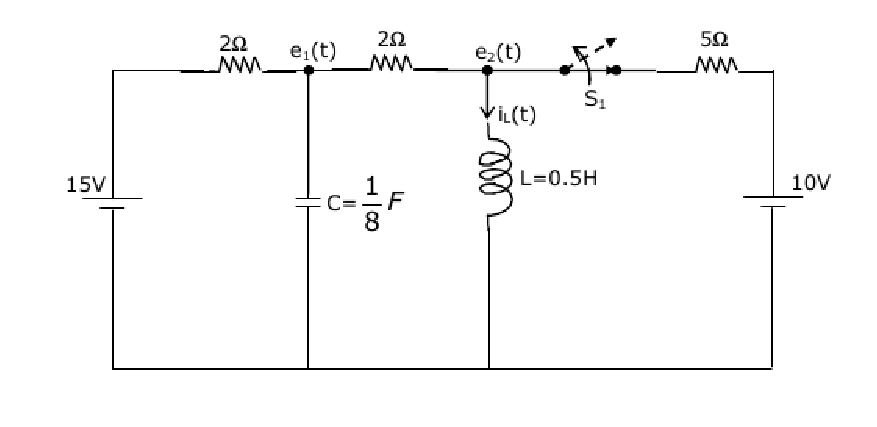
\includegraphics[scale=0.4]{./figs/fig41.eps}
\caption{}
\label{fig41}
\end{center}
\end{figure}
\end{enumerate}

\item The dependent current source shown in figure\ref{fig42} 
\begin{enumerate}
\setlength\itemsep{2em}
\begin{multicols}{2}
\item delivers 80W
\item absorbs 80W
\item delivers 40W
\item absorbs 40W
\end{multicols}
\begin{figure}[!h]
\begin{center}
\includegraphics[scale=0.5]{./figs/fig42.eps}
\caption{}
\label{fig42}
\end{center}
\end{figure}
\end{enumerate}

\item In figure\ref{fig43},the switch was closed for a long time before opening at t=0.the voltage $V_{x}$ at t=$0^{+}$is
\begin{enumerate}
\setlength\itemsep{2em}
\begin{multicols}{2}
\item 25V
\item 50V
\item -50V
\item 0V
\end{multicols}
\begin{figure}[!h]
\begin{center}
\includegraphics[scale=0.5]{./figs/fig43.eps}
\caption{}
\label{fig43}
\end{center}
\end{figure}
\end{enumerate}

\item In the network of figure\ref{fig44},the maximum power is delivered to $R_{L}$ if its value is
\begin{enumerate}
\setlength\itemsep{2em}
\begin{multicols}{4}
\item 16$\Omega$
\item $\frac{40}{3}\Omega$
\item 60$\Omega$
\item 20$\Omega$
\end{multicols}
\begin{figure}[!h]
\begin{center}
\includegraphics[scale=0.5]{./figs/fig44.eps}
\caption{}
\label{fig44}
\end{center}
\end{figure}
\end{enumerate}

\item The switch in Figure.\ref{fig45} has been in position1 for a long time and is then moved to
position2 at t=0.
\begin{enumerate}
\setlength\itemsep{2em}
\item Determine $V_{c}(0^{+})$ and $I_{L}(0^{+})$
\item Determine $\frac{dV_{c}(t)}{dt}$ at t=$0^{+}$
\item Determine $V_{c}(t)$ for $t>0$
\begin{figure}[!h]
\begin{center}
\includegraphics[scale=0.5]{./figs/fig45.eps}
\caption{}
\label{fig45}
\end{center}
\end{figure}
\end{enumerate}

\item For the network shown in Figure.\ref{fig46},R=1 K$\Omega$,$L_{1}$ = 2H, $L_{2}$ = 5H,$L_{3}$ = 1H,$L_{4}$ = 4H and C=0.2$\mu$F.The mutual inductances are $M_{12}$=3H and $M_{34}$=2H. Determine
\begin{enumerate}
\setlength\itemsep{2em}
\item the equivalent inductance for the combination of $L_{3}$and$L_{4}$.
\item the equivalent inductance across the points A and B in the network.
\item the resonant frequency of the network.
\begin{figure}[!h]
\begin{center}
\includegraphics[scale=0.5]{./figs/fig46.eps}
\caption{}
\label{fig46}
\end{center}
\end{figure}
\end{enumerate}


\item The minimum number of equations required to analyze the circuit shown in figure.\ref{fig47}
\begin{enumerate}
\setlength\itemsep{2em}
\begin{multicols}{2}
\item 3
\item 4
\item 6
\item 7
\end{multicols}
\begin{figure}[!h]
\begin{center}
\includegraphics[scale=0.5]{./figs/fig47.eps}
\caption{}
\label{fig47}
\end{center}
\end{figure}
\end{enumerate}

\item A source of angular frequency 1 rad/sec has a source impedance consisting of 1$\Omega$ resistance in series with 1H inductance.The load that will obtain the maximum power transfer is
\begin{enumerate}
\setlength\itemsep{2em}
\item 1$\Omega$ resistance
\item 1$\Omega$ resistance in parallel with 1H inductance
\item 1$\Omega$ resistance in series with 1F capacitor
\item 1$\Omega$ resistance in parallel with 1F capacitor
\end{enumerate}

\item A series RLC circuit has a resonance frequency of 1 kHz and a quality factor Q=100. If each R,L and C is doubled from its original value,the new Q of the circuit  is
\begin{enumerate}
\setlength\itemsep{2em}
\begin{multicols}{4}
\item 25
\item 50
\item 100
\item 200
\end{multicols}
\end{enumerate}

\item The differential equation for the current i(t) in the circiut of figure.\ref{fig48} is
\begin{enumerate}
\setlength\itemsep{2em}
\item 2$\frac{d^{2}i}{dt^{2}}$+2$\frac{di}{dt}$+i(t)=sint
\item $\frac{d^{2}i}{dt^{2}}$+2$\frac{di}{dt}$+2i(t)=cost
\item 2$\frac{d^{2}i}{dt^{2}}$+2$\frac{di}{dt}$+i(t)=cost
\item $\frac{d^{2}i}{dt^{2}}$+2$\frac{di}{dt}$+2i(t)=sint
\begin{figure}[!h]
\begin{center}
\includegraphics[scale=0.7]{./figs/fig48.eps}
\caption{}
\label{fig48}
\end{center}
\end{figure}
\end{enumerate}

\item Twelve 1$\Omega$ resistances are used as edges to form a cube. The resistance between two diagonally opposite corners of the cube is
\begin{enumerate}
\setlength\itemsep{2em}
\begin{multicols}{4}
\item $\frac{5}{6}\Omega$
\item $\frac{1}{6}\Omega$
\item $\frac{6}{5}\Omega$
\item $\frac{3}{2}\Omega$
\end{multicols}
\end{enumerate}

\item The current flowing through the resistance R in the circuit in figure.\ref{fig49} has the form
P cos 4t,where P is
\begin{enumerate}
\setlength\itemsep{2em}
\item (0.18+j0.72)
\item (0.46+j1.90)
\item -(0.18+j1.90)
\item -(0.192+j0.144)

\begin{figure}[!h]
\begin{center}
\includegraphics[scale=0.5]{./figs/fig49.eps}
\caption{}
\label{fig49}
\end{center}
\end{figure}
\end{enumerate}

\item The circuit for Q.55-56 is given in figure.\ref{fig50}. For both the questions, assume that the switch S is in position1 for a long time and thrown to position2 at t=0.At t=$0^{+}$, the current $i_{1}$ is
\begin{enumerate}
\begin{multicols}{2}
\setlength\itemsep{2em}
\item $\frac{-V}{2R}$
\item $\frac{-V}{R}$
\item $\frac{-V}{4R}$
\item zero
\end{multicols}
\begin{figure}[!h]
\begin{center}
\includegraphics[scale=0.5]{./figs/fig50.eps}
\caption{}
\label{fig50}
\end{center}
\end{figure}
\end{enumerate}

\item $I_{1}$(s) and $I_{2}$(s) are the Laplace transforms of $i_{1}$(t) and $i_{2}$(t)respectively.The equations for the loop currents $I_{1}$(s)and $I_{2}$(s) for the circuit shown in figure Q.55-56, after the switch is brought from position1 to position2 at t=0,are
\begin{enumerate}
\setlength\itemsep{2em}
\item $\begin{bmatrix}
R+L_{s}+\frac{1}{C_{s}} & -L_{s}\\
-L_{s} & R+\frac{1}{C_{s}}\\
\end{bmatrix}$
\quad
$\begin{bmatrix}
I_{1}(s)\\
I_{2}(s)
\end{bmatrix}$
\quad =
$\begin{bmatrix}
\frac{V}{s}\\
0
\end{bmatrix}$

\item $\begin{bmatrix}
R+L_{s}+\frac{1}{C_{s}} & -L_{s}\\
-L_{s} & R+\frac{1}{C_{s}}\\
\end{bmatrix}$
\quad
$\begin{bmatrix}
I_{1}(s)\\
I_{2}(s)
\end{bmatrix}$
\quad =
$\begin{bmatrix}
-\frac{V}{s}\\
0
\end{bmatrix}$

\item $\begin{bmatrix}
R+L_{s}+\frac{1}{C_{s}} & -L_{s}\\
-L_{s} & R+L_{s}+\frac{1}{C_{s}}\\
\end{bmatrix}$
\quad
$\begin{bmatrix}
I_{1}(s)\\
I_{2}(s)
\end{bmatrix}$
\quad =
$\begin{bmatrix}
\frac{V}{s}\\
0
\end{bmatrix}$

\item $\begin{bmatrix}
R+L_{s}+\frac{1}{C_{s}} & -L_{s}\\
-L_{s} & R+L_{s}+\frac{1}{C_{s}}\\
\end{bmatrix}$
\quad
$\begin{bmatrix}
I_{1}(s)\\
I_{2}(s)
\end{bmatrix}$
\quad =
$\begin{bmatrix}
-\frac{V}{s}\\
0
\end{bmatrix}$
\end{enumerate}

\item An input voltage v(t)=10$\sqrt{2}$ cos(t+10$^{\circ}$)+10$\sqrt{3}$ cos(2t+10$^{\circ}$)V is applied to a series combination of resistance R=1$\Omega$ and an inductance L=1H. The resulting steady state current i(t) in ampere is
\begin{enumerate}
\setlength\itemsep{2em}
\item 10 cos(t+55$^{\circ}$)+10 cos(2t+10$^{\circ}$+$\tan^{-1}$2)
\item 10 cos(t+55$^{\circ}$)+10$\sqrt{\frac{3}{2}}cos(2t+55^{\circ}$)
\item 10 cos(t-35$^{\circ}$)+10 cos(2t+10$^{\circ}-\tan^{-1}$2)
\item 10 cos(t-35$^{\circ}$)+10$\sqrt{\frac{3}{2}}cos(2t-35^{\circ}$)
\end{enumerate}

\item The equivalent inductance measured between the terminals1 and2 for the circuit shown in figure.\ref{fig51},is
\begin{enumerate}
\setlength\itemsep{2em}
\begin{multicols}{2}
\item $L_{1}$+$L_{2}$+M
\item $L_{1}$+$L_{2}$-M
\item $L_{1}$+$L_{2}$+2M
\item $L_{1}$+$L_{2}$-2M
\end{multicols}
\begin{figure}[!h]
\begin{center}
\includegraphics[scale=0.7]{./figs/fig51.eps}
\caption{}
\label{fig51}
\end{center}
\end{figure}
\end{enumerate}

\item The circuit shown in figure.\ref{fig52} with R=$\frac{1}{3}$W, L=$\frac{1}{4}$H, C=3F has input voltage v(t)=sin2t.The resulting current i(t) is
\begin{enumerate}
\setlength\itemsep{2em}
\begin{multicols}{2}
\item 5sin(2t+53.1$^{\circ}$)
\item 5sin(2t-53.1$^{\circ}$)
\item 25sin(2t+53.1$^{\circ}$)
\item 25sin(2t-53.1$^{\circ}$)
\end{multicols}
\begin{figure}[!h]
\begin{center}
\includegraphics[scale=0.7]{./figs/fig52.eps}
\caption{}
\label{fig52}
\end{center}
\end{figure}
\end{enumerate}

\item For the circuit shown in Figure.\ref{fig53},the time constant RC=1ms.The input voltage is $v_{1}$(t)=$\sqrt{2} sin 10^{3} t$.The output voltage $v_{0}$(t) is equal to
\begin{enumerate}
\setlength\itemsep{2em}
\begin{multicols}{2}
\item sin($10^{3}t-45^{\circ}$)
\item sin($10^{3}t+45^{\circ}$)
\item sin($10^{3}t-53^{\circ}$)
\item sin($10^{3}t+53^{\circ}$)
\end{multicols}
\begin{figure}[!h]
\begin{center}
\includegraphics[scale=0.7]{./figs/fig53.eps}
\caption{}
\label{fig53}
\end{center}
\end{figure}
\end{enumerate}

\item For the R-L circuit shown in Figure.\ref{fig54},the input voltage $v_{i}$(t)=u(t).The current i(t) is
\begin{figure}[!h]
\begin{center}
\includegraphics[scale=0.7]{./figs/fig54a.eps}
\includegraphics[scale=0.7]{./figs/fig54b.eps}
\includegraphics[scale=0.7]{./figs/fig54c.eps}
\includegraphics[scale=0.7]{./figs/fig54d.eps}
\includegraphics[scale=0.7]{./figs/fig54e.eps}
\caption{}
\label{fig54}
\end{center}
\end{figure}

\item The circuit shown in Figure.\ref{fig55} has initial current $i_{L}$(0) = 1A through the inductor
and an initial voltage $V_{c}$(0) = -1V across the capacitor. For input v(t) = u(t), the
Laplace transform of the current i(t) for t$\geq$0 is
\begin{enumerate}
\setlength\itemsep{2em}
\begin{multicols}{4}
\item $\frac{s}{s^{2}+s+1}$
\item $\frac{s+2}{s^{2}+s+1}$
\item $\frac{s-2}{s^{2}+s+1}$
\item $\frac{s-2}{s^{2}+s-1}$
\end{multicols}
\begin{figure}[!h]
\begin{center}
\includegraphics[scale=0.7]{./figs/fig55.eps}
\caption{}
\label{fig55}
\end{center}
\end{figure}
\end{enumerate}

\item For the circuit shown in Figure.\ref{fig56},the initial conditions are zero.Its transfer function H(s)=$\frac{V_{c}(S)}{V_{1}(s)}$ is
\begin{enumerate}
\setlength\itemsep{2em}
\begin{multicols}{2}
\item $\frac{1}{s^{2}+10^{6}s+10^{6}}$
\item $\frac{10^{6}}{s^{2}+10^{3}s+10^{6}}$
\item $\frac{10^{3}}{s^{2}+10^{3}s+10^{6}}$
\item $\frac{10^{6}}{s^{2}+10^{6}s+10^{6}}$
\end{multicols}
\begin{figure}[!h]
\begin{center}
\includegraphics[scale=0.8]{./figs/fig56.eps}
\caption{}
\label{fig56}
\end{center}
\end{figure}
\end{enumerate}

\item The condition on R,L and C such that the step response y(t) in figure.\ref{fig57} has no oscillations,is
\begin{enumerate}
\setlength\itemsep{2em}
\begin{multicols}{2}
\item R$\geq\frac{1}{2}\sqrt{\frac{L}{C}}$
\item R$\geq\sqrt{\frac{L}{C}}$
\item R$\geq2\sqrt{\frac{L}{C}}$
\item R=$\frac{1}{\sqrt{LC}}$
\end{multicols}
\begin{figure}[!h]
\begin{center}
\includegraphics[scale=0.7]{./figs/fig57.eps}
\caption{}
\label{fig57}
\end{center}
\end{figure}
\end{enumerate}

\item In a series RLC circuit R=2k$\Omega$, L=1H and C=$\frac{1}{400}\mu$F.The resonant frequency is
\begin{enumerate}
\setlength\itemsep{2em}
\begin{multicols}{2}
\item 2$\times10^{4}$ Hz
\item $\frac{1}{\pi}\times10^{4}$ Hz
\item $10^{4}$ Hz
\item 2$\pi\times10^{4}$ Hz
\end{multicols}
\end{enumerate}

\item The maximum power that can be transferred to the load resistor $ R_{L}$ from the
voltage source in figure.\ref{fig58} is
\begin{enumerate}
\setlength\itemsep{2em}
\begin{multicols}{4}
\item 1W 
\item 10W
\item 0.25W
\item 0.5W
\end{multicols}
\begin{figure}[!h]
\begin{center}
\includegraphics[scale=0.8]{./figs/fig58.eps}
\caption{}
\label{fig58}
\end{center}
\end{figure}
\end{enumerate}

\item For the circuit in figure.\ref{fig59} the instantaneous current $i_{1}$(t) is
\begin{enumerate}
\setlength\itemsep{2em}
\begin{multicols}{2}
\item $\frac{10\sqrt{3}}{2}\angle90^\circ$ Amps
\item $\frac{10\sqrt{3}}{2}\angle-90^\circ$ Amps
\item 5$\angle60^\circ$ Amps
\item 5$\angle-60^\circ$ Amps
\end{multicols}
\begin{figure}[!h]
\begin{center}
\includegraphics[scale=0.7]{./figs/fig59.eps}
\caption{}
\label{fig59}
\end{center}
\end{figure}
\end{enumerate}

\item Impedance Z as shown in figure.\ref{fig60} is:
\begin{enumerate}
\setlength\itemsep{2em}
\begin{multicols}{2}
\item j29$\Omega$ 
\item j9$\Omega$
\item j19$\Omega$
\item j39$\Omega$
\end{multicols}
\begin{figure}[!h]
\begin{center}
\includegraphics[scale=0.5]{./figs/fig60.eps}
\caption{}
\label{fig60}
\end{center}
\end{figure}
\end{enumerate}

\item For the circuit shown in figure.\ref{fig61},Thevenin’s voltage and 
\begin{enumerate}
\setlength\itemsep{2em}
\begin{multicols}{2}
\item 5V and 2$\Omega$
\item 7.5V and 2.5$\Omega$
\item 4V and 2$\Omega$
\item 3V and 2.5$\Omega$
\end{multicols}
\begin{figure}[!h]
\begin{center}
\includegraphics[scale=0.5]{./figs/fig61.eps}
\caption{}
\label{fig61}
\end{center}
\end{figure}
\end{enumerate}



\item If $R_{1}$=$R_{2}$=$R_{4}$and$R_{3}$ = 1. 1R in the bridge circuit shown in figure.\ref{fig62}, then the reading in the ideal voltmeter connected between a and b is
\begin{enumerate}
\setlength\itemsep{2em}
\begin{multicols}{2}
\item 0.238 V
\item 0.138 V 
\item -0.238 V
\item 1 V
\end{multicols}
\begin{figure}[!h]
\begin{center}
\includegraphics[scale=0.5]{./figs/fig62.eps}
\caption{}
\label{fig62}
\end{center}
\end{figure}
\end{enumerate}

\item A square pulse of 3 volts amplitude is applied to C-R circuit shown in figure.\ref{fig63}. The
capacitor is initially uncharged. The ouput voltage $v_{0}$ at time t=2 sec is
\begin{enumerate}
\setlength\itemsep{2em}
\begin{multicols}{4}
\item 3V
\item -3V 
\item  4V
\item -4V
\end{multicols}
\begin{figure}[!h]
\begin{center}
\includegraphics[scale=0.5]{./figs/fig63.eps}
\caption{}
\label{fig63}
\end{center}
\end{figure}
\end{enumerate}


\item In the figure.\ref{fig64} shown below, assume that all the capacitors are initially uncharged.
If $v_{i}$(t)=10u(t) Volts, $v_{0}$(t) is given by
\begin{enumerate}
\setlength\itemsep{2em}
\begin{multicols}{2}
\item 8$e^{-0.004t}$ Volts
\item 8$(1-e^{-0.004t})$
\item 8u(t) Volts 
\item 8 Volts
\end{multicols}
\begin{figure}[!h]
\begin{center}
\includegraphics[scale=0.4]{./figs/fig64.eps}
\caption{}
\label{fig64}
\end{center}
\end{figure}
\end{enumerate}


\item The RC circuit shown in the figure.\ref{fig65} is
\begin{enumerate}
\setlength\itemsep{2em}
\begin{multicols}{2}
\item a low-pass filter
\item a high-pass filter
\item a band-pass filter 
\item a band-reject filter
\end{multicols}
\begin{figure}[!h]
\begin{center}
\includegraphics[scale=0.7]{./figs/fig65.eps}
\caption{}
\label{fig65}
\end{center}
\end{figure}
\end{enumerate}

\item Two series resonant filters are as shown in the figure.\ref{fig66}. Let the 3-dB bandwidth of
Filter1 be $B_{1}$ and that of Filter2 be $B_{2}$.The value of $\frac{B_{1}}{B_{2}}$ is:
\begin{enumerate}
\setlength\itemsep{2em}
\begin{multicols}{4}
\item 4
\item 1
\item $\frac{1}{2}$
\item $ \frac{1}{4} $
\end{multicols}
\begin{figure}[!h]
\begin{center}
\includegraphics[scale=0.5]{./figs/fig66.eps}
\caption{}
\label{fig66}
\end{center}
\end{figure}
\end{enumerate}

\item For the circuit shown in the figure.\ref{fig67}, the Thevenin voltage and resistance looking into X-Y
\begin{enumerate}
\setlength\itemsep{2em}
\begin{multicols}{2}
\item $\frac{4}{3}$V,2$\Omega$ 
\item 4V,$ \frac{2}{3}\Omega $
\item $ \frac{4}{3} $V,$ \frac{2}{3} \Omega$
\item 4V,2$ \Omega $
\end{multicols}
\begin{figure}[!h]
\begin{center}
\includegraphics[scale=0.7]{./figs/fig67.eps}
\caption{}
\label{fig67}
\end{center}
\end{figure}
\end{enumerate}

\item In the circuit shown in figure.\ref{fig68}, $V_{c}$is 0 volts at t=0 sec. For t$ > $0,the capacitor current
$i_{c}(t)$ , where t is in seconds, is given by
\begin{enumerate}
\setlength\itemsep{2em}
\begin{multicols}{2}
\item 0.50 exp(-25t)mA
\item 0.25 exp(-25t)mA
\item 0.50 exp(-12.5t)mA
\item 0.25 exp(-6.25t)mA
\end{multicols}
\begin{figure}[!h]
\begin{center}
\includegraphics[scale=0.7]{./figs/fig68.eps}
\caption{}
\label{fig68}
\end{center}
\end{figure}
\end{enumerate}

\item In the AC network shown in the figure.\ref{fig69},the phasor voltage $V_{AB}$(in Volts) is:
\begin{enumerate}
\setlength\itemsep{2em}
\item 0
\item 5$\angle30 ^\circ$
\item 12.5$\angle30^\circ$
\item 17$\angle30^\circ$
\begin{figure}[!h]
\begin{center}
\includegraphics[scale=0.8]{./figs/fig69.eps}
\caption{}
\label{fig69}
\end{center}
\end{figure}
\end{enumerate}


\item  The Thevenin’s equivalent impedance $Z_{TH}$ between the nodes P and Q in the following figure.\ref{fig70} is
\begin{enumerate}
\setlength\itemsep{2em}
\begin{multicols}{4}
\item 1
\item 1+s+$\frac{1}{s}$
\item 2+s+$\frac{1}{s}$
\item $\frac{s^{2}+s+1}{s^{2}+2s+1}$
\end{multicols}
\begin{figure}[!h]
\begin{center}
\includegraphics[scale=0.7]{./figs/fig70.eps}
\caption{}
\label{fig70}
\end{center}
\end{figure}
\end{enumerate}

\item The driving point impedance of the following figure.\ref{fig71} is given by Z(s)=$\frac{0.2s}{s^{2}+0.1s+2}$.The component values are
\begin{enumerate}
\setlength\itemsep{2em}
\item L=5H, R=0.5$\Omega$, C=0.1F
\item L=0.1H, R=0.5$\Omega$, C=5F
\item L=0.1H, R=2$\Omega$, C=0.1F
\item L=0.1H, R=2$\Omega$, C=5F
\begin{figure}[!h]
\begin{center}
\includegraphics[scale=0.5]{./figs/fig71.eps}
\caption{}
\label{fig71}
\end{center}
\end{figure}
\end{enumerate}

\item The circuit shown in the figure.\ref{fig72} is used to charge the capacitor C alternately from two current sources as indicated. The switches S1 and S2 are mechanically coupled and connected as follows
\begin{enumerate}
\setlength\itemsep{2em}
\item For 2nT$\leq$t$<$(2n+1)T ;(n=0,1,2..)S1 to P1 and S2 to P2
 \item For (2n+1)T$\leq$t$<$(2n+2)T, (n=0,1,2....)S1 to Q1 and S2 to Q2
 Assume that the capacitor has zero initial charge.Given that u(t) is a unit step function,the voltage$ V_{c}(t) $ across the capacitor is given by
 \begin{enumerate}[(A)]
 \item $ \Sigma_{n=0}^{\infty} (-1)^{n} tu(t-nT)$
 \item u(t) + 2 $ \Sigma_{n=1}^{\infty} (-1)^{n} u(t-nT)$
 \item tu(t) + 2 $ \Sigma_{n=1}^{\infty} (-1)^{n} (t-nT) u(t-nT)$
 \item $\Sigma_{n=0}^{\infty}[0.5 - e^-({t-2nt})+0.5e^-({t-2nT-T})]$
 
\end{enumerate}
\begin{figure}[!h]
\begin{center}
\includegraphics[scale=0.7]{./figs/fig72.eps}
\caption{}
\label{fig72}
\end{center}
\end{figure}
\end{enumerate}

\item For t$>$0,the output voltage $V_{c}$(t) is
\begin{enumerate}
\setlength\itemsep{2em}
\item $\frac{2}{\sqrt{3}}(e^{-\frac{1}{2}}t-e^{\frac{-\sqrt{3}}{2}}$t)
\item $\frac{2}{\sqrt{3}}te^{-\frac{1}{2}}$t
\item $ \frac{2}{\sqrt{3}}e^{-\frac{1}{2}}t cos(\frac{\sqrt{3}}{2}t)$
\item $ \frac{2}{\sqrt{3}}e^{-\frac{t}{2}} sin(\frac{\sqrt{3}}{2}t)$
\end{enumerate}

\item For t$>$0, the voltage across the resistor is
\begin{enumerate}
\setlength\itemsep{2em}
\item $\frac{1}{\sqrt{3}}(e^{\frac{-\sqrt{3}}{2}t}-e^{-\frac{1}{2}t})$
\item e$\frac{-1}{2}t[cos (\frac{\sqrt{3t}}{2})-\frac{1}{\sqrt{3}}sin(\frac{\sqrt{3t}}{2})]$
\item $ \frac{2}{\sqrt{3}}e^-{\frac{1}{2}t}sin(\frac{\sqrt{3t}}{2}) $
\item $ \frac{2}{\sqrt{3}}e^-{\frac{1}{2}t}cos(\frac{\sqrt{3t}}{2}) $
\end{enumerate}


\item If the transfer function of the following figure.\ref{fig73} is $\frac{V_{0}(s)}{V_{1}(s)}$=$\frac{1}{2+s^{CR}}$ the value of the load resistance $R_{L}$ is
\begin{enumerate}
\setlength\itemsep{2em}
\begin{multicols}{2}
\item  $\frac{R}{4}$
\item $ \frac{R}{2} $
\item R
\item 2R
\end{multicols}
\begin{figure}[!h]
\begin{center}
\includegraphics[scale=0.9]{./figs/fig73.eps}
\caption{}
\label{fig73}
\end{center}
\end{figure}
\end{enumerate}
 
\item The switch in the figure.\ref{fig74} shown was on position a for a long time and is moved to position b at time t=0 .The current i(t) for t$>0$ is given by
\begin{enumerate}
\setlength\itemsep{2em}
\begin{multicols}{2}
\item  0.2$e^{-125t}$u(t) mA
\item 20$e^{-1250t}$u(t) mA
\item 0.2$e^{-1250t}$u(t) mA
\item 20$e^{-1000t}$u(t) mA
\end{multicols}
\begin{figure}[!h]
\begin{center}
\includegraphics[scale=0.9]{./figs/fig74.eps}
\caption{}
\label{fig74}
\end{center}
\end{figure}
\end{enumerate}

\item  In the figure.\ref{fig75} shown ,what value of $R_{L}$ maximizes the power delivered to $R_{L}$ ?
\begin{enumerate}
\setlength\itemsep{2em}
\begin{multicols}{2}
\item 2.4$\Omega$
\item $\frac{8}{3}\Omega$
\item 4$\Omega$
\item 6$\Omega$
\end{multicols}
\begin{figure}[!h]
\begin{center}
\includegraphics[scale=0.9]{./figs/fig75.eps}
\caption{}
\label{fig75}
\end{center}
\end{figure}
\end{enumerate}

\item The time domain behaviour of an RL circuit is represented by\\ L$\frac{d_{i}} {d_{t}}$+ $R_{i}$ = $V_{0}(1+Be^{-\frac{R_{t}}{L}}sint)$ u(t).\\For an initial current of i(0)=$\frac{V_{0}}{R}$,the steady state value of the current is given by
\begin{enumerate}
\setlength\itemsep{2em}
\begin{multicols}{2}
\item i(t)$\rightarrow\frac{V_{0}}{R}$
\item i(t)$\rightarrow\frac{2V_{0}}{R}$
\item i(t)$\rightarrow\frac{V_{0}}{R}$(1+B)
\item i(t)$\rightarrow\frac{2V_{0}}{R}$(1+B)
\end{multicols}
\end{enumerate}

\item For parallel RLC circuit, which one of the following statements is NOT correct?
\begin{enumerate}
\setlength\itemsep{2em}
\item The bandwidth of the circuit decreases if R is increased.
\item The bandwidth of the circuit remains same if L is increased.
\item At resonance, input impedance is a real quantity.
\item At resonance, the magnitude of input impedance attains its minimum value.
\end{enumerate}

\item In the figure.\ref{fig76} shown, the switch S is open for a long time and is closed at t=0. The
current i(t) for t$\geq0^{+}$ is
\begin{enumerate}
\setlength\itemsep{2em}
\item i(t)=$0.5-0.125e^{-1000t}$A
\item i(t)=$1.5-0.125e^{-1000t}$A.
\item i(t)=$0.5-0.5e^{-1000t}$A
\item i(t)=$0.375e^{-1000t}$A
\begin{figure}[!h]
\begin{center}
\includegraphics[scale=0.5]{./figs/fig76.eps}
\caption{}
\label{fig76}
\end{center}
\end{figure}
\end{enumerate}

\item The current I in the figure.\ref{fig77} shown is
\begin{enumerate}
\setlength\itemsep{2em}
\begin{multicols}{4}
\item -j1A
\item J1A
\item 0A
\item 20A
\end{multicols}
\begin{figure}[!h]
\begin{center}
\includegraphics[scale=0.5]{./figs/fig77.eps}
\caption{}
\label{fig77}
\end{center}
\end{figure}
\end{enumerate}

\item In the figure.\ref{fig78}shown,the power supplied by the voltage source is
\begin{enumerate}
\setlength\itemsep{2em}
\item 0W
\item 5W
\item 10w
\item 100w
\begin{figure}[!h]
\begin{center}
\includegraphics[scale=0.5]{./figs/fig78.eps}
\caption{}
\label{fig78}
\end{center}
\end{figure}
\end{enumerate}


\item The figure.\ref{fig79} shown below is driven by a sinusoidal input $ V_{i} $ = $V_{p}cos(\frac{t}{RC})$ .The steady state output $V_{0}$ is
\begin{enumerate}
\setlength\itemsep{2em}
\begin{multicols}{2}
\item $ (\frac{V_{p}}{3})cos(\frac{t}{RC}) $
\item $ (\frac{V_{p}}{3})sin(\frac{t}{RC}) $
\item $ (\frac{V_{p}}{2})cos(\frac{t}{RC}) $
\item $ (\frac{V_{p}}{2})sin(\frac{t}{RC}) $
\end{multicols}
\begin{figure}[!h]
\begin{center}
\includegraphics[scale=0.7]{./figs/fig79.eps}
\caption{}
\label{fig79}
\end{center}
\end{figure}
\end{enumerate}

\item In the figure.\ref{fig80} shown below, the Norton equivalent current in amperes with respect
to the terminals P and Q is
\begin{enumerate}
\begin{multicols}{2}
\setlength\itemsep{2em}
\item 6.4-j4.8
\item 6.56-j7.87
\item 10+j0
\item 16+j0
\end{multicols}
\begin{figure}[!h]
\begin{center}
\includegraphics[scale=0.7]{./figs/fig80.eps}
\caption{}
\label{fig80}
\end{center}
\end{figure}
\end{enumerate}

\item In the figure.\ref{fig81}shown below, the value of $ R_{L} $ such that the power transferred to $ R_{L} $ is maximum
\begin{enumerate}
\setlength\itemsep{2em}
\begin{multicols}{2}
\item 5$ \Omega $
\item 10$ \Omega $
\item 15$ \Omega $
\item 20$ \Omega $
\end{multicols}
\begin{figure}[!h]
\begin{center}
\includegraphics[scale=0.7]{./figs/fig81.eps}
\caption{}
\label{fig81}
\end{center}
\end{figure}
\end{enumerate}

\item In the figure.\ref{fig82} shown below, the current I is equal to
\begin{enumerate}
\setlength\itemsep{2em}
\begin{multicols}{2}
\item 14$\angle 0^{\circ}$A
\item 2.0$\angle 0^{\circ}$A
\item 2.8$\angle 0^{\circ}$A
\item 3.2$\angle 0^{\circ}$A
\end{multicols}
\begin{figure}[!h]
\begin{center}
\includegraphics[scale=0.7]{./figs/fig82.eps}
\caption{}
\label{fig82}
\end{center}
\end{figure}
\end{enumerate}

\item In the figure.\ref{fig83} shown below, the initial charge on the capacitor is 2.5 mC, with the
voltage polarity as indicated. The switch is closed at time t=0. The current i(t) at
a time t after the switch is closed is
\begin{enumerate}
\setlength\itemsep{2em}
\item i(t)=15exp(-2$\times10^{3}$t)A
\item i(t)=5exp(-2$\times10^{3}$t)A
\item i(t)=10exp(-2$\times10^{3}$t)A
\item i(t)=-5exp(-2$\times10^{3}$t)A
\begin{figure}[!h]
\begin{center}
\includegraphics[scale=0.7]{./figs/fig83.eps}
\caption{}
\label{fig83}
\end{center}
\end{figure}
\end{enumerate}


\item In the figure.\ref{fig84} shown below,the current through the inductor is
\begin{enumerate}
\setlength\itemsep{2em}
\begin{multicols}{2}
\item $\frac{2}{1+j}$A
\item $\frac{-1}{1+j}$A
\item $\frac{1}{1+j}$A
\item 0A
\end{multicols}
\begin{figure}[!h]
\begin{center}
\includegraphics[scale=0.7]{./figs/fig84.eps}
\caption{}
\label{fig84}
\end{center}
\end{figure}
\end{enumerate}

\item The impedance looking into nodes 1 and 2 in the given figure.\ref{fig85} is
\begin{enumerate}
\setlength\itemsep{2em}
\begin{multicols}{4}
\item 50$ \Omega $
\item 100$ \Omega $
\item 5K$ \Omega $
\item 10.1k$ \Omega $
\end{multicols}
\begin{figure}[!h]
\begin{center}
\includegraphics[scale=0.5]{./figs/fig85.eps}
\caption{}
\label{fig85}
\end{center}
\end{figure}
\end{enumerate}


\item In the following figure $ C_{1} $ and$ C_{2} $ are ideal capacitors.$ C_{1} $ has been charged to 12V before the ideal switch S is closed at t=0.The figure.\ref{fig86} i(t) for all t is 
\begin{enumerate}
\setlength\itemsep{2em}
\item zero
\item a step function
\item an exponentially decaying function
\item an impulse function
\begin{figure}[!h]
\begin{center}
\includegraphics[scale=0.7]{./figs/fig86.eps}
\caption{}
\label{fig86}
\end{center}
\end{figure}
\end{enumerate}

\item If $ V_{A} $ - $ V_{B} $=6V,then $ V_{C} $ - $ V_{D} $ is, figure.\ref{fig87}
\begin{enumerate}
\begin{multicols}{4}
\setlength\itemsep{2em}
\item -5V
\item 2V
\item 3V
\item 6V
\end{multicols}
\begin{figure}[!h]
\begin{center}
\includegraphics[scale=0.9]{./figs/fig87.eps}
\caption{}
\label{fig87}
\end{center}
\end{figure}
\end{enumerate}

\item Assuming both the voltages sources are in phase,the value of R for which maximum power is transfered from circuit A to circuit B is,figure.\ref{fig88}
\begin{enumerate}
\begin{multicols}{2}
\setlength\itemsep{2em}
\item 0.8$ \Omega $
\item 1.4$ \Omega $
\item 2$ \Omega $
\item 2.8$ \Omega $
\end{multicols}
\begin{figure}[!h]
\begin{center}
\includegraphics[scale=0.7]{./figs/fig88.eps}
\caption{}
\label{fig88}
\end{center}
\end{figure}
\end{enumerate}


\item The transfer function $ \frac{V_{2}(s)}{V_{1}(s)} $ of the figure.\ref{fig89}shown below is
\begin{enumerate}
\begin{multicols}{2}
\setlength\itemsep{2em}
\item $ \frac{0.5s+1}{s+1} $
\item $ \frac{3s+6}{s+2} $
\item $ \frac{s+2}{s+1} $
\item $ \frac{s+1}{s+2} $
\end{multicols}
\begin{figure}[!h]
\begin{center}
\includegraphics[scale=0.7]{./figs/fig89.eps}
\caption{}
\label{fig89}
\end{center}
\end{figure}
\end{enumerate}

\item In the circuit shown below, if the source voltage $V_{s}$= 100 $\angle$ 53.13$^\circ$V then the Thevenin’s equivalent voltage in Volts as seen by the load resistance $R^{L}$ is
\begin{enumerate}
\begin{multicols}{2}
\setlength\itemsep{2em}
\item 100$\angle$90$^\circ$
\item 800$\angle$0$^\circ$
\item 800$\angle$90$^\circ$
\item 100$\angle$60$^\circ$
\end{multicols}
\begin{figure}[!h]
\begin{center}
\includegraphics[scale=0.4]{./figs/fig90.eps}
\caption{}
\label{fig90}
\end{center}
\end{figure}
\end{enumerate}
 
\item Consider the following figure.\ref{fig91} for question (a) and (b).
\begin{figure}[!h]
\begin{center}
\includegraphics[scale=0.7]{./figs/fig91.eps}
\caption{}
\label{fig91}
\end{center}
\end{figure}

\begin{enumerate}
 
\item  The current $ I_{s} $ in Amps in the voltage source, and voltage $ V_{s} $ in Volts across the current source respectively, are
\begin{enumerate}
\begin{multicols}{2}
\setlength\itemsep{2em}
\item 13,-20
\item 8,-10
\item -8,20
\item -13,20
\end{multicols}
\end{enumerate}

\item The current in the 1$ \Omega $ resistor in Amps is,
\begin{enumerate}
\begin{multicols}{4}
\setlength\itemsep{2em}
\item 2
\item 3.33
\item 10
\item 12
\end{multicols}
\end{enumerate}
\end{enumerate}


\item Find the current I in the following Branch.,figure.\ref{fig92}
\begin{figure}[!h]
\begin{center}
\includegraphics[scale=0.5]{./figs/fig92.eps}
\caption{}
\label{fig92}
\end{center}
\end{figure}

\item A series $R_{c}$ figure.\ref{fig93} is connected to DC voltage source at time $t_{0}$=0.The relation between the source voltage $V_{s}$,the resistance R,the capacitance C,the current i(t) is below:\\ \\
$V_{s}$= $R_{i}(t)$ + $\frac{1}{C}\int_{0}^{t}$i(t)dt.\\ \\Which one of the following i(t) represents
\begin{figure}[!h]
\begin{center}
\includegraphics[scale=0.4]{./figs/fig93a.eps}
\includegraphics[scale=0.4]{./figs/fig93b.eps}
\includegraphics[scale=0.4]{./figs/fig93c.eps}
\includegraphics[scale=0.4]{./figs/fig93d.eps}
\caption{}
\label{fig93}
\end{center}
\end{figure}

\item Find the resistance $R_{1}$ from y figure.\ref{fig94}
\begin{figure}[!h]
\begin{center}
\includegraphics[scale=0.7]{./figs/fig94.eps}
\caption{}
\label{fig94}
\end{center}
\end{figure}

\item Find the $ V_{0} $,figure.\ref{fig95}\\
\begin{enumerate}
\setlength\itemsep{2em}
\item $\frac{5}{2}V_{1}$-3$V_{2}$
\item 2$V_{1}$-$\frac{5}{2}V_{2}$
\item $\frac{-3}{2}V_{1}$-$\frac{7}{2}V_{2}$
\item -3$V_{1}+\frac{11}{2}V_{2}$
\begin{figure}[!h]
\begin{center}
\includegraphics[scale=0.7]{./figs/fig95.eps}
\caption{}
\label{fig95}
\end{center}
\end{figure}
\end{enumerate}

 
\item For the figure.\ref{fig96} given below, what will be the largest value of arm when it is
converted into delta form.
\begin{figure}[!h]
\begin{center}
\includegraphics[scale=0.7]{./figs/fig96.eps}
\caption{}
\label{fig96}
\end{center}
\end{figure}

\item For the given figure.\ref{fig97}, the value of capacitor is in mF. So that the system will
be critically damped is
\begin{figure}[!h]
\begin{center}
\includegraphics[scale=0.7]{./figs/fig97.eps}
\caption{}
\label{fig97}
\end{center}
\end{figure}

\item Where R=1$ \Omega $,$ i_{1} $ = 2A, $ i_{4} $ = –1A, $ i_{5} $ = –4A. Then which of the following is correct,figure.\ref{fig98}
\begin{enumerate}
\setlength\itemsep{2em}
\item $ i_{6} $=5A
\item $ i_{3} $=-4A
\item Given data sufficient to tell these currents are not possible
\item Data is not sufficeint to find $ i_{2} $,$ i_{3} $,$ i_{6} $
\begin{figure}[!h]
\begin{center}
\includegraphics[scale=0.7]{./figs/fig98.eps}
\caption{}
\label{fig98}
\end{center}
\end{figure}
\end{enumerate}


\item In the figure.\ref{fig99} shown,at resonance,the amplitude of the sinusoidal voltage(in Volts) across the capacitor is
\begin{figure}[!h]
\begin{center}
\includegraphics[scale=0.7]{./figs/fig99.eps}
\caption{}
\label{fig99}
\end{center}
\end{figure}

\item In the network shown in the figure.\ref{fig100}, all resistors are identical with R=300$ \Omega $. The resistance $ R_{ab} $ (in $ \Omega $) of the network is
\begin{figure}[!h]
\begin{center}
\includegraphics[scale=0.5]{./figs/fig100.eps}
\includegraphics[scale=0.7]{./figs/fig100a.eps}
\caption{}
\label{fig100}
\end{center}
\end{figure}

\item In the given figure.\ref{fig101}, the values of $ V_{1} $ and $ V_{2} $ respectively are
\begin{enumerate}
\setlength\itemsep{2em}
\begin{multicols}{2}
\item 5V,25V
\item 10V,30V
\item 15V,35V
\item 0V,20V
\end{multicols}
\begin{figure}[!h]
\begin{center}
\includegraphics[scale=0.7]{./figs/fig101.eps}
\caption{}
\label{fig101}
\end{center}
\end{figure}
\end{enumerate}


\item In the figure.\ref{fig102} shown, the switch SW is thrown from positionA to positionB at time t=0. The energy (in $ \mu $J) taken from the 3V source to charge the 0.1 $\mu$F capacitor from 0V to 3V is
\begin{enumerate}
\setlength\itemsep{2em}
\begin{multicols}{4}
\item 0.3
\item 0.45
\item 0.9
\item 3
\end{multicols}
\begin{figure}[!h]
\begin{center}
\includegraphics[scale=0.7]{./figs/fig102.eps}
\caption{}
\label{fig102}
\end{center}
\end{figure}
\end{enumerate}

\item The damping ratio of a series RLC circuit can be expressed as
\begin{enumerate}
\setlength\itemsep{2em}
\begin{multicols}{2}
\item $\frac{R^{2}C}{2L}$
\item $\frac{2L}{R^{2}C}$
\item $\frac{R}{2}\sqrt{\frac{C}{L}}$
\item $\frac{2}{R}\sqrt{\frac{L}{C}}$
\end{multicols}
\end{enumerate}

\item In the figure.\ref{fig103} shown, switch SW is closed at t=0. Assuming zero initial conditions, the value of $V_{c}$(t)(in Volts) at t=1 sec is
\begin{figure}[!h]
\begin{center}
\includegraphics[scale=0.5]{./figs/fig103.eps}
\caption{}
\label{fig103}
\end{center}
\end{figure}

\item In the given figure.\ref{fig104}, the maximum power (in Watts) that can be transferred to the load $R_{L}$ is
\begin{figure}[!h]
\begin{center}
\includegraphics[scale=0.4]{./figs/fig104.eps}
\caption{}
\label{fig104}
\end{center}
\end{figure}

 
\item The Venn diagram.\ref{fig105} shows the preference of the student population for leisure activities.From the data given,the number of students who like to read books or play sports is
\begin{enumerate}
\setlength\itemsep{2em}
\begin{multicols}{4}
\item 44
\item 51
\item 79
\item 108
\end{multicols}
\begin{figure}[!h]
\begin{center}
\includegraphics[scale=0.5]{./figs/fig105.eps}
\caption{}
\label{fig105}
\end{center}
\end{figure}
\end{enumerate}

\item Social science disciplines were in existence in an amorphous form until the colonial period when they were institutionalized. In varying degrees, they were intended to further the colonial interest.In the time of globalization and the economic rise of postcolonial countries like India,conventional ways of knowledge production have become obsolete.\\
  
  Which of the following can be logically inferred from the above statements?
  \begin{enumerate}[(i)]
\item Social science disciplines have become obsolete.
\item Social science disciplines had a pre-colonial origin.
\item Social science disciplines always promote colonialism.
\item Social science must maintain disciplinary boundaries.
\end{enumerate}
\begin{enumerate}[A]
\begin{multicols}{2}
\item (ii)only
\item (i) and (iii) only
\item (ii) and (iv) only
\item (iii) and (iv) only
\end{multicols}
\end{enumerate}

\item Two and a quarter hours back, when seen in a mirror, the reflection of a wall clock without number markings seemed to show 1:30.What is the actual current time shown by the clock?
\begin{enumerate}
\setlength\itemsep{2em}
\begin{multicols}{4}
\item 8:15
\item 11:15
\item 12:15
\item 12:45
\end{multicols}
\end{enumerate}

\item In the given circuit.\ref{fig106}, each resistor has a value equal to 1$ \Omega $
What is the equivalent resistance across the terminals a and b?
\begin{figure}[!h]
\begin{center}
\includegraphics[scale=0.5]{./figs/fig106.eps}
\caption{}
\label{fig106}
\end{center}
\end{figure}

\begin{enumerate}
\setlength\itemsep{2em}
\begin{multicols}{4}
\item $\frac{1}{6} \Omega $
\item $\frac{1}{3} \Omega $
\item $\frac{9}{20} \Omega $
\item $\frac{8}{15} \Omega $
\end{multicols}
\end{enumerate}

\item In the circuit shown in the figure.\ref{fig107}, the magnitude of the current (in amperes) through $R_{2}$ is
\begin{figure}[!h]
\begin{center}
\includegraphics[scale=0.5]{./figs/fig107.eps}
\caption{}
\label{fig107}
\end{center}
\end{figure}



\item In the circuit.\ref{fig108} shown,V is a sinusoidal voltage source.The current I is in phase with voltage V.\\The ratio $\frac{amplitude \ of\  voltage\ across\ the\ capacitor}{amplitude\ of\ voltage\ across\ the\ resistor}$ is
\begin{figure}[!h]
\begin{center}
\includegraphics[scale=0.7]{./figs/fig108.eps}
\caption{}
\label{fig108}
\end{center}
\end{figure}

\item The switch in the circuit.\ref{fig109} shown in the figure was open for a long time and is closed at t=0.The current i(t) (in ampere) at t=0.5 seconds
\begin{figure}[!h]
\begin{center}
\includegraphics[scale=0.5]{./figs/fig109.eps}
\caption{}
\label{fig109}
\end{center}
\end{figure}

\item Consider the circuit shown in the figure.\ref{fig110}. The Thevenin equivalent resistance (in$ \Omega $)across P-Q is
\begin{figure}[!h]
\begin{center}
\includegraphics[scale=0.4]{./figs/fig110.eps}
\caption{}
\label{fig110}
\end{center}
\end{figure}

























































































\end{enumerate}
\end{document}
